\subsection{Signal strength}
\label{subsec:signalstrenghts}

A simultaneous fit to all categories is performed to extract the signal-strength modifier,
defined as the ratio of the observed H boson rate in the $\mathrm{H}\rightarrow{\rm Z}{\rm Z}\rightarrow4\ell$ decay channel to the standard model expectation.

All measurements are reported at $\mH=125.38$ GeV, the best mass obtained by CMS from the combination of $H\rightarrow$~ZZ and $H\rightarrow\gamma\gamma$ channels.

The combined measurement of the inclusive signal-strength modifier is: % with $\mH$ profiled in the fit is
$\mu = 0.94~^{+0.11}_{-0.12} = 0.94^{+0.07}_{-0.07}~({\rm stat})~^{+0.09}_{-0.08}~({\rm syst})$.
%\begin{align}
%    \label{eqn:muinclusive}
%    \mu &= 0.96~^{+0.11}_{-0.10} \\
%    \nonumber &= 0.96^{+0.07}_{-0.07}~({\rm stat})~^{+0.09}_{-0.07}~({\rm syst})~.
%\end{align}
The dominant experimental sources of systematic uncertainty are the uncertainties in the lepton identification efficiencies and luminosity measurement, while the dominant theoretical source is the uncertainty in the total gluon fusion cross section.
The contributions to the total uncertainty from experimental and theoretical sources are found to be similar in magnitude.
The signal-strength modifiers are further studied in terms of the five main SM Higgs boson production mechanisms, namely $\mu_{\Pg\Pg\PH,\bbH}$, $\mu_{\mathrm{VBF}}$, $\mu_{\ZH}$, $\mu_{\WH}$, and $\mu_{\ttH,\tH}$.
%The WH and ZH processes are merged into VH.
Contributions of the $\bbH$ and $\tH$ production modes are also taken into account in the fit.
The $\bbH$ contribution is floated together with gluon fusion and $\tH$ production mode is floated with $\ttH$.
The results are shown in Fig.~\ref{fig:mucat} reporting the observed and expected profile likelihood scans of the inclusive signal-strength modifier (left) and the results of likelihood scans for the signal-strength modifiers of the five main SM Higgs boson production mechanisms (right).
The corresponding numerical values, including the decomposition of the uncertainties into statistical and systematic components, and the corresponding expected uncertainties, are given in Table~\ref{tab:sigstr}.

%%%%%%%%%%%%%%%%%%%%%%%
\begin{figure}[!htb]
\begin{center}
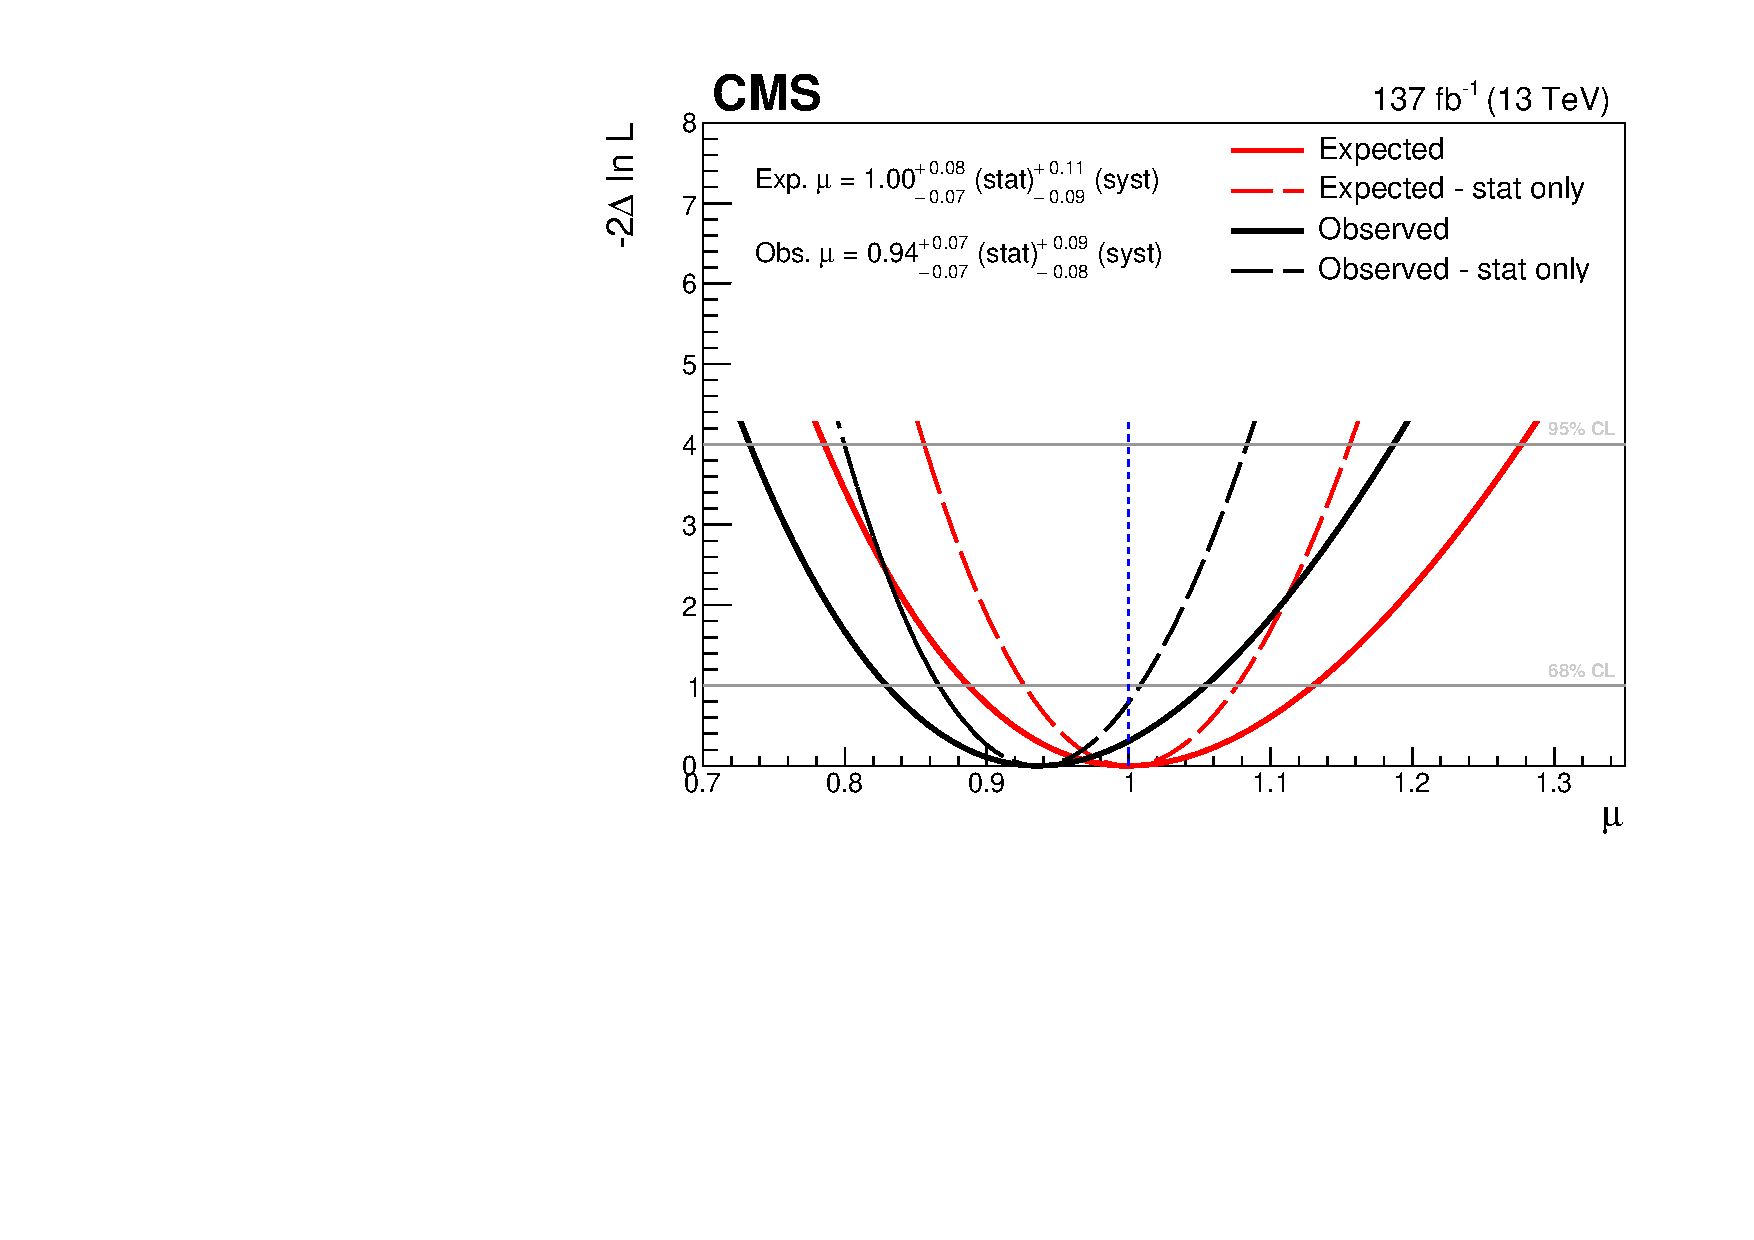
\includegraphics[width=0.49\linewidth]{Figures/results/signalstrength/InclusiveMu_125_38.pdf}
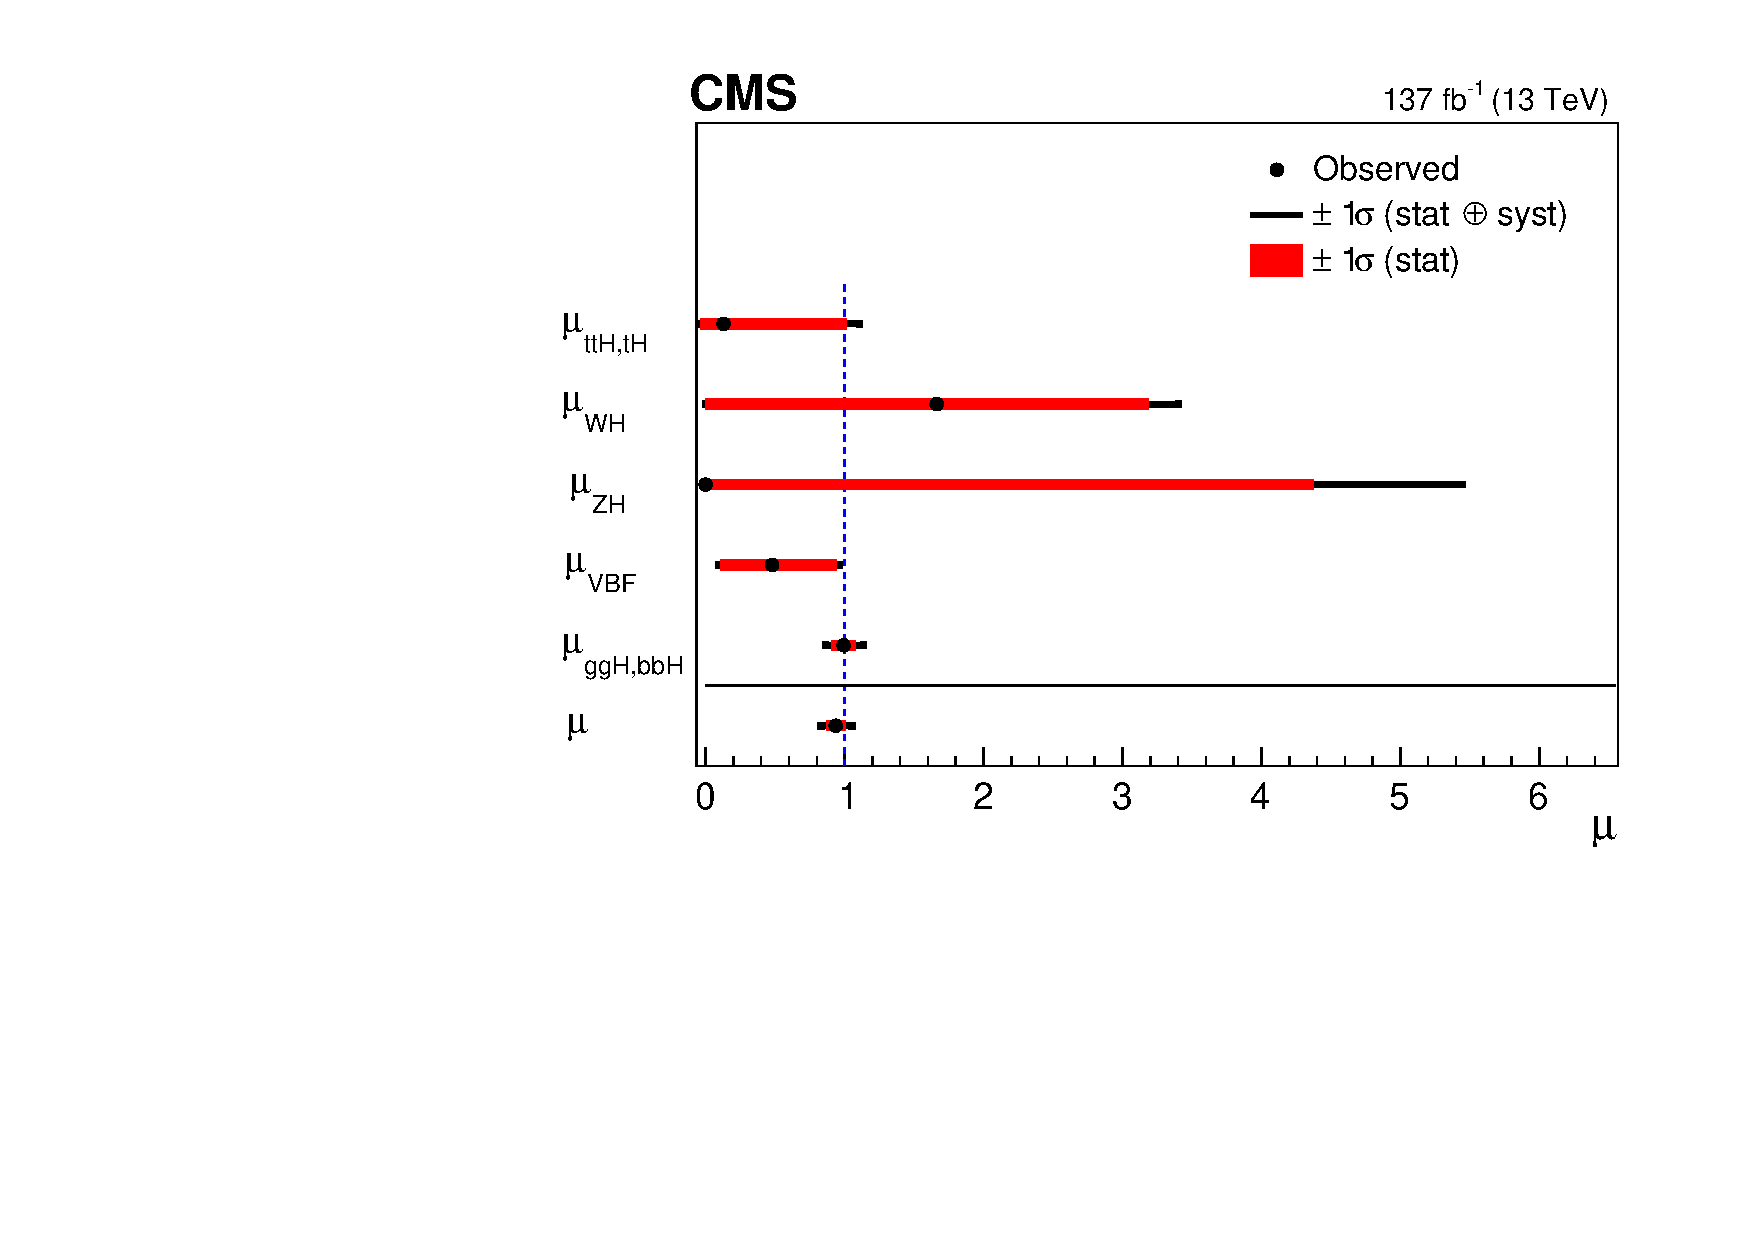
\includegraphics[width=0.49\linewidth]{Figures/results/signalstrength/mu_stage0_125_38.pdf}
\caption{
(Left) The observed and expected profile likelihood scans of the inclusive signal-strength modifier. The scans are shown both with (solid line) and without (dashed line) systematic uncertainties.
(Right) Results of likelihood scans for the signal-strength modifiers corresponding to the five main SM Higgs boson production mechanisms, compared to the inclusive signal strength modifier  $\mu$ shown as a vertical line.
The thick black lines report the $1\sigma$ confidence intervals including both statistical and systematic sources.
The thick red lines report the statistical uncertainties of the $1\sigma$ confidence intervals.
\label{fig:mucat}}
\end{center}
\end{figure}
%%%%%%%%%%%%%%%%%%%%%%%

\begin{table}[hb]
	\begin{center}
		\caption{
		Best-fit values and $\pm 1\sigma$ uncertainties for the expected and observed signal-strength modifiers.
		The uncertainty numbers are broken into statistical and systematic sources.
		The expected results are obtained for $\mH=125.38~\mathrm{GeV}$. %the observed results are obtained with $\mH$ profiled in the fit.
		\label{tab:sigstr}
			}
    \renewcommand{\arraystretch}{1.5}
    \begin{tabular}{ccc}
	\hline
	& Expected & Observed \\
	\hline
	$\mu_{\Pg\Pg\PH,\bbH}$ & $1.00~^{+0.10}_{-0.10}$~(stat)$~^ {+0.12}_{-0.10}~$(syst) & $0.99 ^{+0.09 }_{-0.09}$(stat)~$~^ {+0.11}_{-0.09}~$(syst) \\
  $\mu_{\mathrm{VBF}}$ & $1.00~^{+0.53}_{-0.44}$~(stat)$~^ {+0.18}_{-0.12}~$(syst) & $0.48 ^{+0.46}_{-0.37}$(stat)~$~^ {+0.14}_{-0.10}~$(syst) \\
  $\mu_{\ZH}$ & $1.00~^{+4.79}_{-1.00}~$(stat)$~^ {+6.76}_{-0.00}~$(syst) & $0. ^{+4.38}_{-0.00}$(stat)~$~^ {+3.24}_{-0.00}~$(syst) \\
  $\mu_{\WH}$ & $1.00~^{+1.83}_{-1.00}~$(stat)$~^{+0.75}_{-0.00}~$(syst) & $1.66 ^{+1.52}_{-1.66}$(stat)~$~^ {+0.85}_{-0.00}~$(syst) \\
	$\mu_{\ttH,\tH}$ & $1.00~^{+1.23}_{-0.77}~$(stat)$~^ {+0.51}_{-0.06}~$(syst) & $0.17 ^{+0.88}_{-0.17}$(stat)~$~^{+0.42}_{-0.00}~$(syst) \\
		  	\hline
	$\mu$ & $1.00~^{+0.08}_{-0.07}$~(stat)~$^{+0.10}_{-0.08}$~(syst) & $0.94~^{+0.07}_{-0.07}$~(stat)~$^{+0.09}_{-0.08}$~(syst)\\
	\hline
\end{tabular}
	\end{center}
\end{table}

Two signal strength modifiers $\muF$ and $\muV$ are introduced as scale factors for the fermion- and vector-boson induced contribution to the expected SM cross section.
A two-parameter fit is performed simultaneously to all reconstructed event categories, leading to the measurements of $\muF=\valMuF$ and $\muV=\valMuV$. 
%profiling $\mH$, 
The expected meaurements obtained for $\mH=125.38~\mathrm{GeV}$ are $\muF~=~1.00~^{+0.15}_{-0.13}$ and $\muV~=~1.00~^{+0.39}_{-0.33}$.
The 68\% and 95\%~CL contours in the ($\muF,\muV$) plane are shown in Fig.~\ref{fig:mu2D} and the SM predictions lie within the 68\%~CL regions of this measurement.

% %%%%%%%%%%%%%%%%%%%%%%%
\begin{figure}[!htb]
\begin{center}
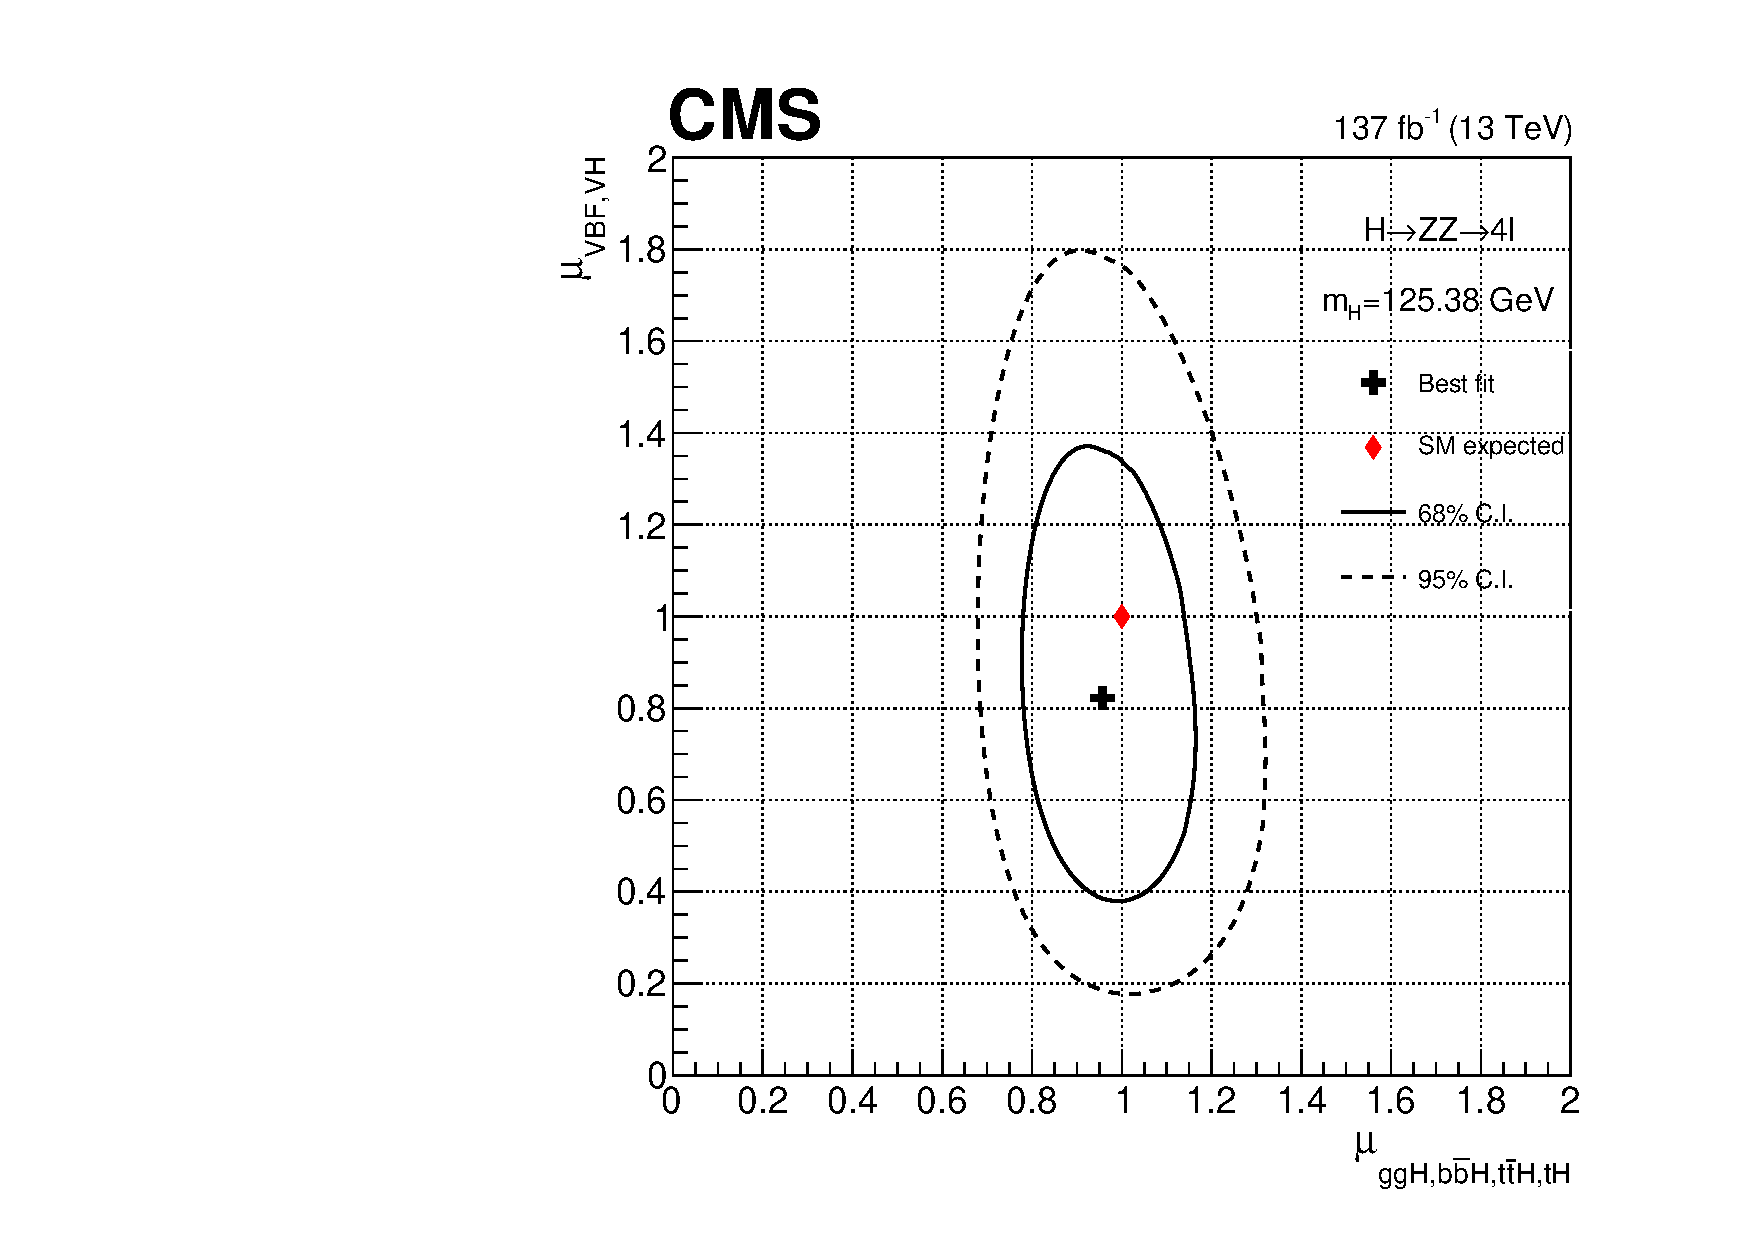
\includegraphics[width=0.9\linewidth]{Figures/results/signalstrength/rvrf_125_38.pdf}
\caption{
Result of the 2D likelihood scan for the $\muF$ and $\muV$ signal-strength modifiers.
The solid and dashed contours show the 68\% and 95\% CL regions, respectively.
The cross indicates the best-fit value, and the diamond represents the expected value for the SM Higgs boson.
\label{fig:mu2D}}
\end{center}
\end{figure}
% %%%%%%%%%%%%%%%%%%%%%%%






% OLD text

%\textbf{FIXME: Results shown here used 2017 yield parameterization and categorization but systematics, templates, etc... from 2016 analysis}
%With a 2D fit, the signal strength is measured to be $\mu = 0.98^{+0.11}_{-0.10}$  for a fixed mass hypothesis of $\mH=125~\GeV$. %.09~\GeV$
% (and $X.XX^{+X.XX}_{-X.XX}$ when constraining the Higgs boson mass to $\mH = 125.09\pm0.24\GeV$) 
 %for the inclusive event sample. The results are compared to the expected signal-strength modifiers in Table~\ref{tab:sigstr}.

%{\renewcommand{\arraystretch}{1.2}
%\begin{table}[!hb]
%\begin{center}
%\caption{ Expected and observed signal-strength modifiers. \textbf{FIXME: Numbers to be split by syst/stat uncertainties}
%\label{tab:sigstr}}
%\begin{tabular}{l|c|ccccc}
%   &  Inclusive & $\mu_{\Pg\Pg\PH}$ & $\mu_{\mathrm{VBF}}$ &  $\mu_{\rm VHhad}$ & $\mu_{\rm VHlep}$ & $\mu_{\ttH}$ \\
%\hline
%Expected  & $1.00^{+0.15}_{-0.14}({\rm stat.})^{+0.10}_{-0.09}({\rm sys.})$ & $1.00^{+0.24}_{-0.21}$ & $1.00^{+0.25}_{-0.97}$ & $1.00^{+3.97}_{-1.00}$  & $1.00^{+3.93}_{-1.00}$ & $1.00^{+3.22}_{-1.00}$ \\
%Expected &  $1.00^{+0.17}_{-0.15}$ & $1.00^{+0.21}_{-0.19}$ & $1.00^{+1.11}_{-0.85}$ & $1.00^{+3.84}_{-1.00}$  & $1.00^{+2.86}_{-1.00}$ & $1.00^{+2.50}_{-1.00}$ \\
%Observed  & $XX^{+XX}_{-XX}({\rm stat.})^{+XX}_{XX}({\rm sys.})$ & $XX^{XX}_{XX}$ & $XX^{XX}_{XX}$  & $XX^{+XX}_{-XX}$ & $0.00^{+XX}_{-XX}$ &  $0.00^{+XX}_{-XX}$ \\
%\hline
%\end{tabular}
%\end{center}
%\end{table}
%}

%{\renewcommand{\arraystretch}{1.2}
%\begin{table}[!hb]
%\begin{center}
%\caption{ Expected and observed signal-strength modifiers with 2D scan (with kinematic discriminant).
%\label{tab:sigstr}}
%\resizebox{\textwidth}{!}{\begin{tabular}{l|c|ccccc}
%   &  Inclusive & $\mu_{\Pg\Pg\PH}$ & $\mu_{\mathrm{VBF}}$ &  $\mu_{\rm VH}$ & $\mu_{\ttH}$\\
%\hline
%Expected  & $1.00^{+0.12}_{-0.10}$ & $1.00^{+0.14}_{-0.12}$ & $1.00^{+0.60}_{-0.47}$  & ${1.00}^{+1.09}_{-0.82}$ & $1.00^{+1.17}_{-0.72}$ \\
%Observed  & $0.97^{+0.11}_{-0.10}$ & ${0.67}^{+0.51}_{-0.39}$ & ${0.67}^{+0.51}_{-0.39}$  & ${1.21}^{+1.08}_{-0.85}$ & ${0.33}^{+0.91}_{-0.33}$\\

%\hline
%\end{tabular}}
%\end{center}
%\end{table}
%}


%\begin{figure}[htb]
%\begin{center}
%\includegraphics[width=0.6\linewidth]{Figures/Results/signalstrength/signal_strength_categories_unblind_2017.pdf}
%\caption{Values of $\mu=\sigma/\sigma_{SM}$ for the six categories. 
%The vertical line shows the combined $\mu$, together with its associated $\pm$ 1$\sigma$ uncertainties shown as filled band.  
%The horizontal bars indicate the $\pm$ 1$\sigma$ uncertainties on $\mu$ for the different categories. 
%The uncertainties include both statistical and systematic sources.
%\label{fig:mucat}}
%\end{center}
%\end{figure}

% TO BE ADDED. COMMENTED FOR NOW
%Two signal-strength modifiers $\muF$ and $\muV$ are introduced as scale factors for the fermion and vector-boson induced contribution to the expected SM cross section.
%A two-dimensional fit is performed, profiling the likelihood for all nuisance parameters including the \mH, leading to the measurements of  $\muF=0.98^{+0.13}_{-0.12}$ and $\muV=0.85^{+0.37}_{-0.30}$.
%The 68\% and 95\% CL contours in the ($\muF,\muV$) plane are shown in Fig.~\ref{fig:RVRF}. 
%When constraining the Higgs boson mass to $\mH = 125.09\pm0.24\GeV$ instead of fixing it, the best fit values are $\muF=X.XX$ and $\muV=X.XX$.
%All results for $\mu$, $\muF$ and $\muV$ are reported in Tables~\ref{tab:muvalues_exp} and~\ref{tab:muvalues_obs}.

%\begin{figure}[htb]
%\begin{center}
%    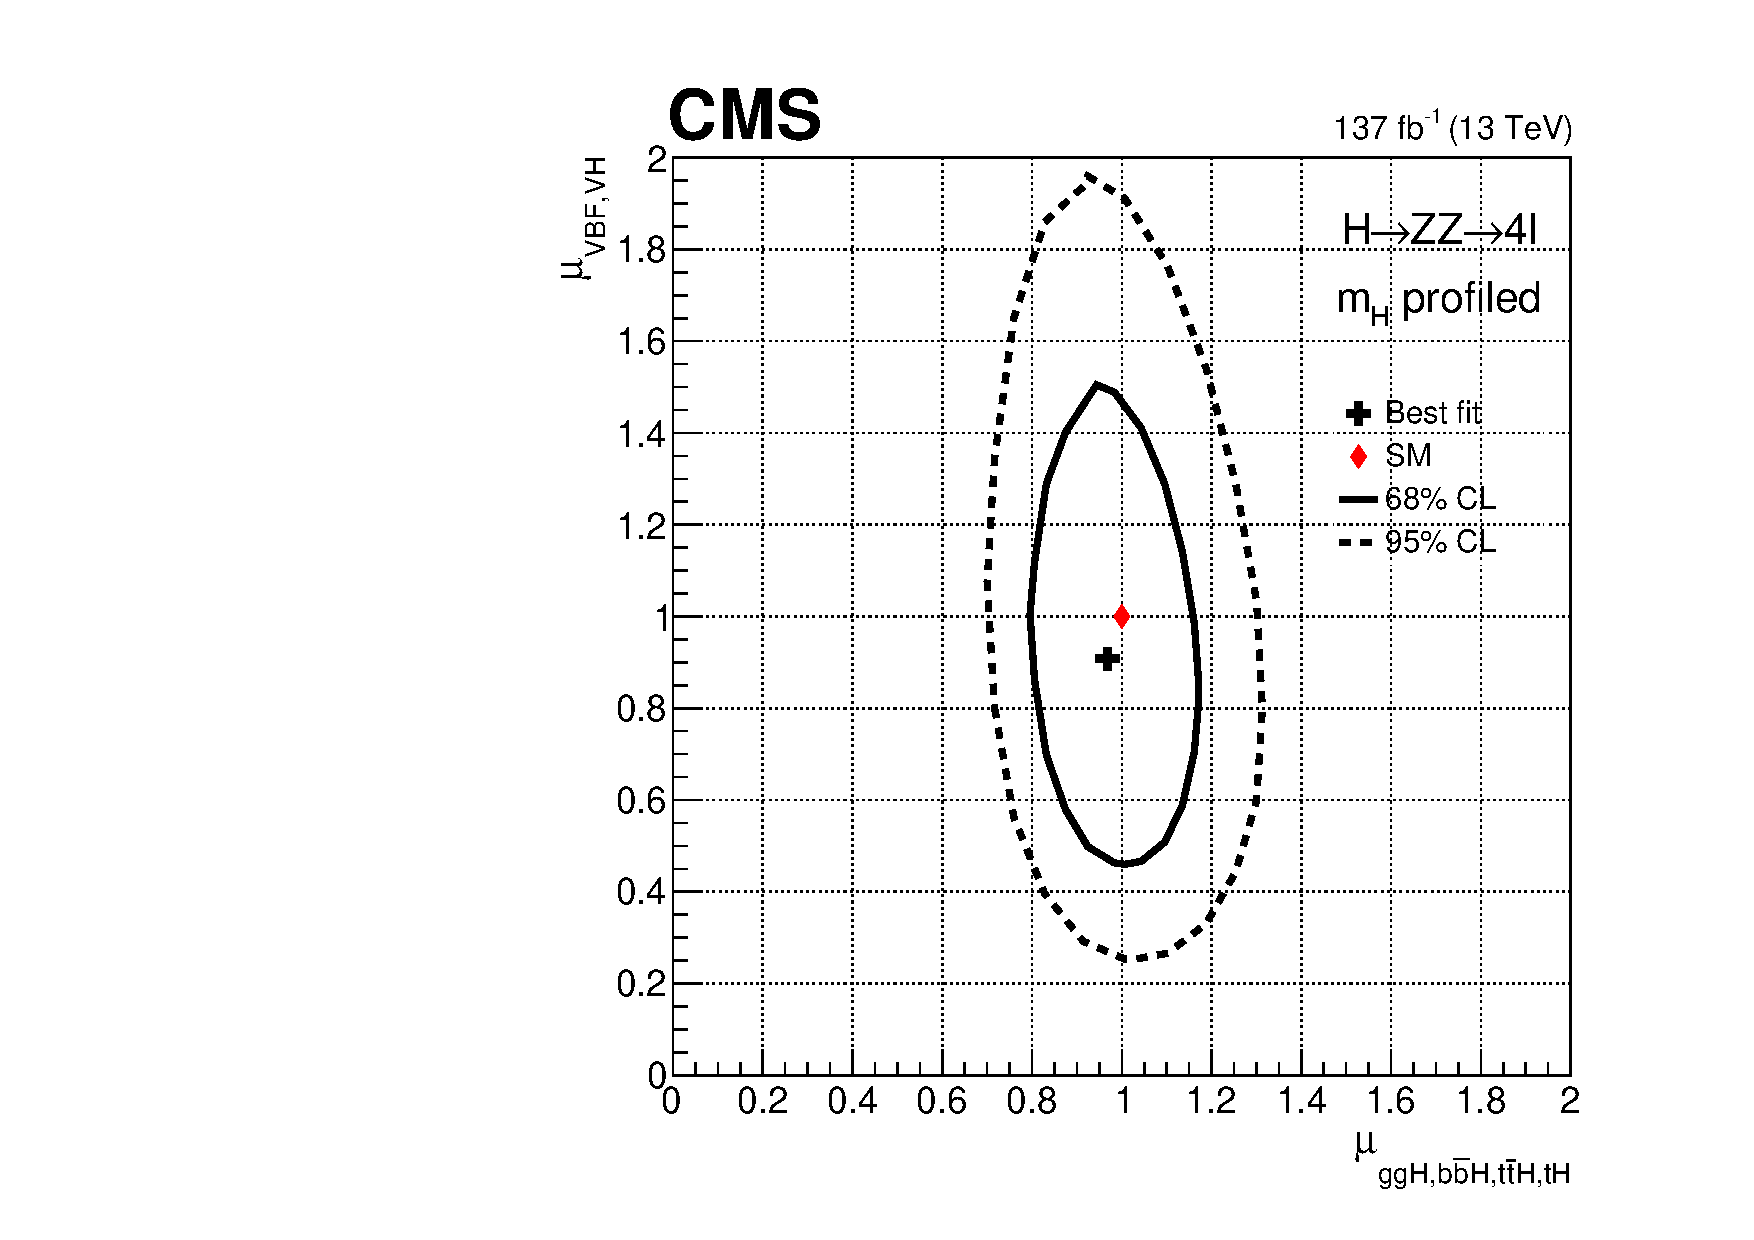
\includegraphics[width=0.6\linewidth]{Figures/results/signalstrength/rvrf.pdf}
%    \caption{ Result of the 2D likelihood scan for the $\muF$ and $\muV$ signal-strength modifiers. 
%   The solid and dashed contours show the 68\% and 95\% CL regions, respectively. 
%    The cross indicates the best-fit values, and the diamond represents the expected values for the SM Higgs boson.
%\label{fig:RVRF}}
%\end{center}
%\end{figure}


%{\renewcommand{\arraystretch}{1.5}
%%%============
%\begin{table}[!hb]
%\begin{center}
%\caption{Expected signal strength values for different measurement setups.
%\label{tab:muvalues_exp}}
%\begin{tabular}{lcccc}
%\hline  
% Categorization  & 1D: ${\cal L}(m_{4l})$ & 2D: ${\cal L}(m_{4l},\KD)$ &   1D: ${\cal L}(m_{4l}')$ & 2D: ${\cal L}(m_{4l}',\KD)$ \\ \hline 
%Inclusive &  $\mu=$1.000$^{+XX}_{-XX}$ & $\mu=$1.000$^{+XX}_{-XX}$ &  $\mu=$1.000$^{+XX}_{-XX}$ & $\mu=$1.000$^{+XX}_{-XX}$ \\ \hline
% &  $\mu=$1.000$^{+XX}_{-XX}$ & $\mu=$1.000$^{+XX}_{-XX}$ &  $\mu=$1.000$^{+XX}_{-XX}$ & $\mu=$1.000$^{+XX}_{-XX}$ \\
%Two categories & $\muV$=1.000$^{+XX}_{-XX}$ & $\muV=$1.000$^{+XX}_{-XX}$ &  $\muV=$1.000$^{+XX}_{-XX}$ & $\muV=$1.000$^{+XX}_{-XX}$ \\
% & $\muF=$1.000$^{+XX}_{-XX}$ & $\muF=$1.000$^{+XX}_{-XX}$ &  $\muF=$1.000$^{+XX}_{-XX}$ & $\muF=$1.000$^{+XX}_{-XX}$ \\
%\hline
%\end{tabular}
%\end{center}
%\end{table}
%%%============
%}
%
%{\renewcommand{\arraystretch}{1.5}
%%%============
%\begin{table}[!hb]
%\begin{center}
%\caption{Expected and observed signal strength values for different measurement setups.
%\label{tab:muvalues_obs}}
%\begin{tabular}{lcccc}
%\hline  
% Categorization  & 1D: ${\cal L}(m_{4l})$ & 2D: ${\cal L}(m_{4l},\KD)$ &   1D: ${\cal L}(m_{4l}')$ & 2D: ${\cal L}(m_{4l}',\KD)$ \\ \hline 
%Inclusive &  $\mu=$X.XX$^{+XX}_{-XX}$ & $\mu=$X.XX$^{+XX}_{-XX}$ &  $\mu=$X.XX$^{+XX}_{-0.XX}$ & $\mu=$X.XX$^{+XX}_{-XX}$ \\ \hline
% &  $\mu=$X.XX$^{+XX}_{-XX}$ & $\mu=$X.XX$^{+XX}_{-XX}$ &  $\mu=$X.XX$^{+XX}_{-XX}$ & $\mu=$X.XX$^{+XX}_{-XX}$ \\
%Two categories & $\muV$=X.XX$^{+XX}_{-XX}$ & $\muV=$X.XX$^{+XX}_{-XX}$ &  $\muV=$X.XX$^{+XX}_{-XX}$ & $\muV=$X.XX$^{+XX}_{-XX}$ \\
% & $\muF=$X.XX$^{+XX}_{-XX}$ & $\muF=$X.XX$^{+XX}_{-XX}$ &  $\muF=$X.XX$^{+XX}_{-XX}$ & $\muF=$X.XX$^{+XX}_{-XX}$ \\
%\hline
%\end{tabular}
%\end{center}
%\end{table}
%%%============
%}

%Signal-strength modifiers for the five main Higgs production modes, $\mu_{\Pg\Pg\PH}$, $\mu_{\mathrm{VBF}}$, $\mu_{\WH}$, $\mu_{\ZH}$ and $\mu_{\ttH}$ are also introduced as scale factors to the expected SM cross section. 
%Similarly, the fits are performed fixing the mass to $\mH = 125~\GeV$ and profiling the likelihood for all nuisance parameters, leading to the results 
%reported in Table~\ref{tab:muprocesses} and 
%illustrated in Fig.~\ref{fig:muprocesses},
% Three models are tested, 
% in Fig.~\ref{fig:muprocesses}(top left) $\mu_{\WH}$ are $\mu_{\ZH}$ are separated, 
% in Fig.~\ref{fig:muprocesses}(top right) $\mu_{\WH}$ are $\mu_{\ZH}$ are grouped in $\mu_{\VH}$, 
% and in Fig.~\ref{fig:muprocesses}(bottom) 
%where $\mu_{\WH}$ and  $\mu_{\ZH}$ are merged to $\mu_{VH}$.
%splitted in the leptonically decay bosons  $\mu_{\WH lep}$/$\mu_{\ZH lep}$ and hadronically decay  bosons $\mu_{\WH lep}$/$\mu_{\ZH lep}$.


%%%============
%\begin{table}[hb]
%\begin{center}
%\caption{Expected and observed results of likelihood scans for the signal strength modifiers corresponding to the five main Higgs boson production modes.
%\label{tab:muprocesses}}
%\begin{tabular}{l|c|c}
%\hline
%   & Expected & Observed  \\
%\hline
%$\mu_{\Pg\Pg\PH}$  & 1.00$^{+0.48}_{-0.43}$ & 1.09$^{+0.47}_{-0.42}$  \\
%$\mu_{\mathrm{VBF}}$  & 1.00$^{+2.51}_{-1.00}$ & 0.00$^{+0.59}_{-0.00}$  \\
%$\mu_{\WH}$  & 1.00$^{+9.20}_{-1.00}$ & 0.00$^{+8.49}_{0.00}$  \\
%$\mu_{\ZH}$  & 1.00$^{+17.96}_{-1.00}$ & 2.48$^{+17.43}_{-2.48}$  \\
%$\mu_{\ttH}$  & 1.00$^{+8.01}_{-1.00}$ & 8.83$^{+16.39}_{-8.83}$ \\
%\hline
%\end{tabular}
%\end{center}
%\end{table}
%%%============

%\begin{figure}[htb]
%\begin{center}
% \includegraphics[width=0.45\linewidth]{Figures/Results/signalstrength/compatibility_process_ZHWH.pdf}
% \includegraphics[width=0.45\linewidth]{Figures/Results/signalstrength/compatibility_process_VH.pdf} \\
%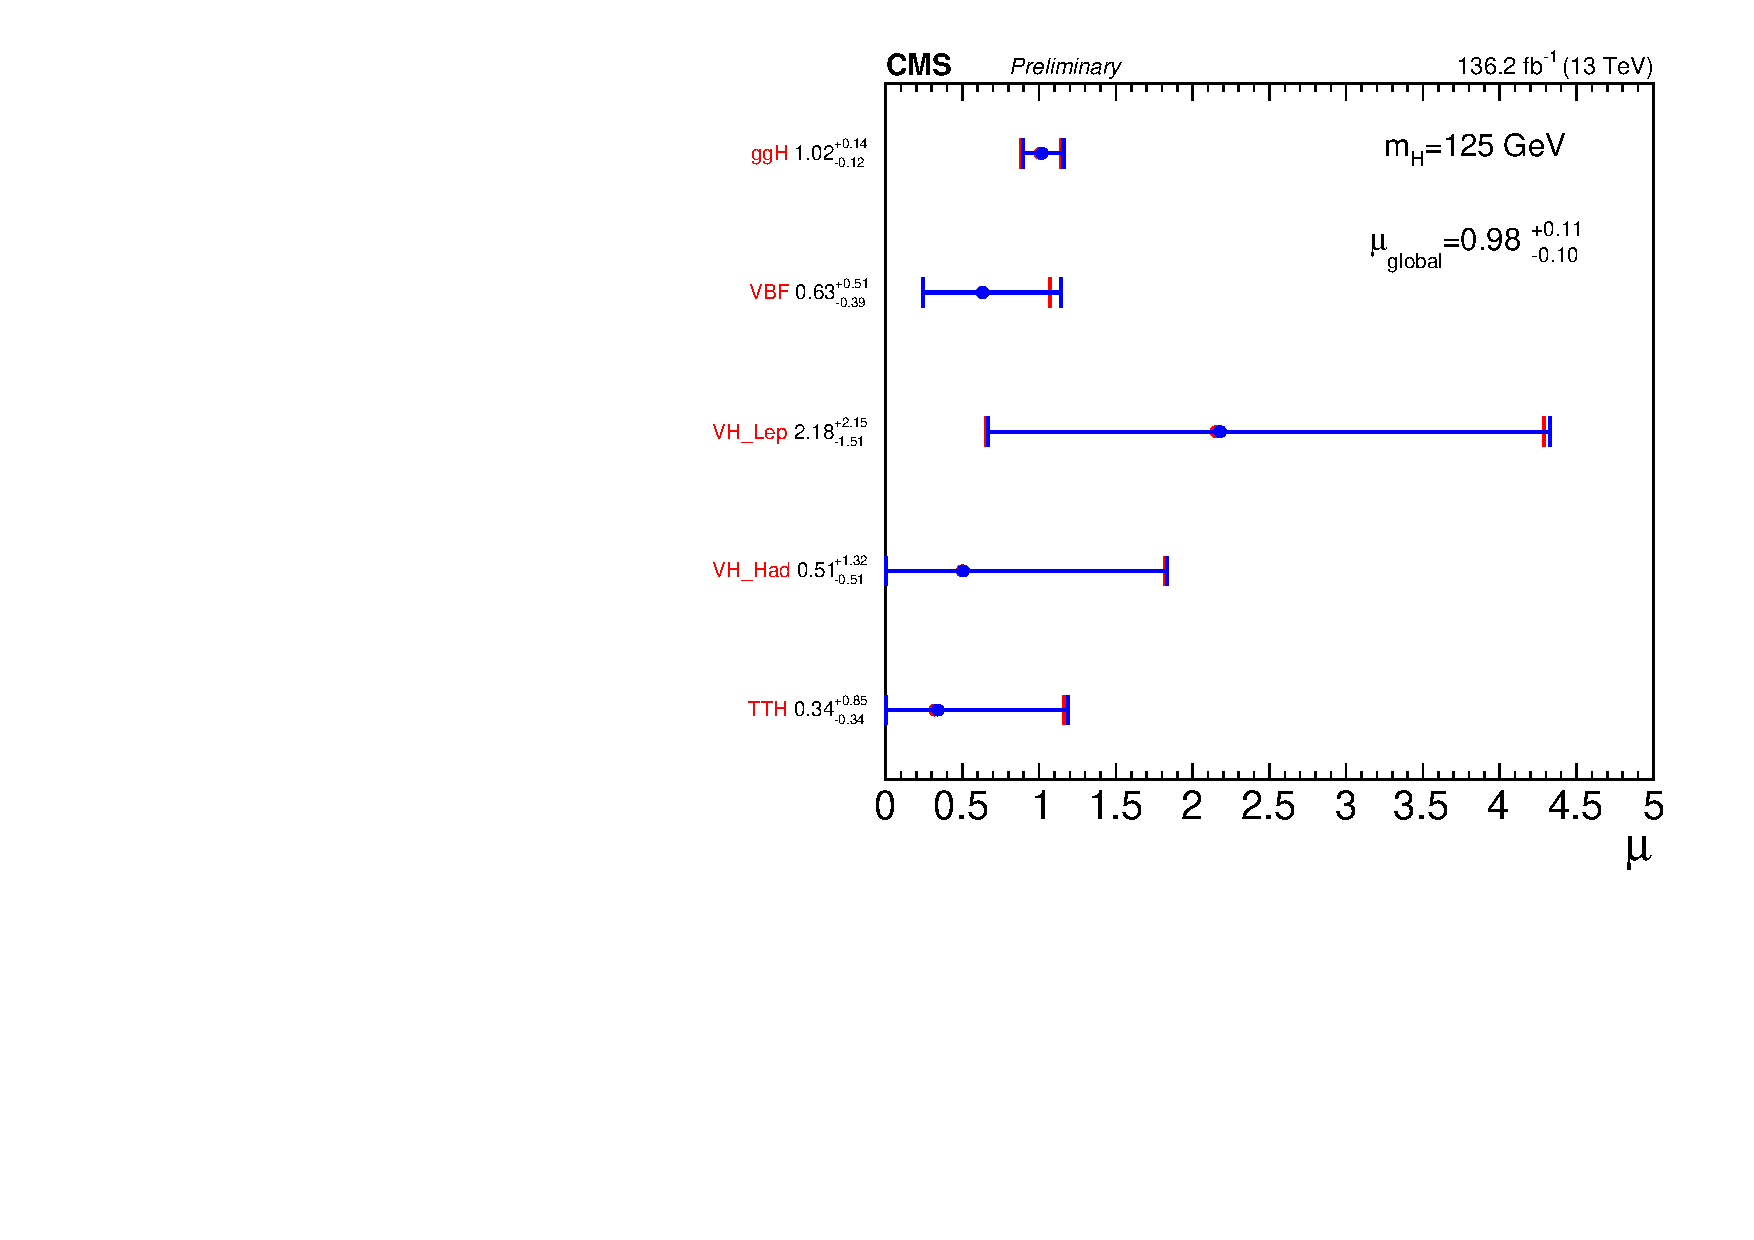
\includegraphics[width=0.80\linewidth]{Figures/results/signalstrength/mu_stage0_hadlep1_obs.pdf}
%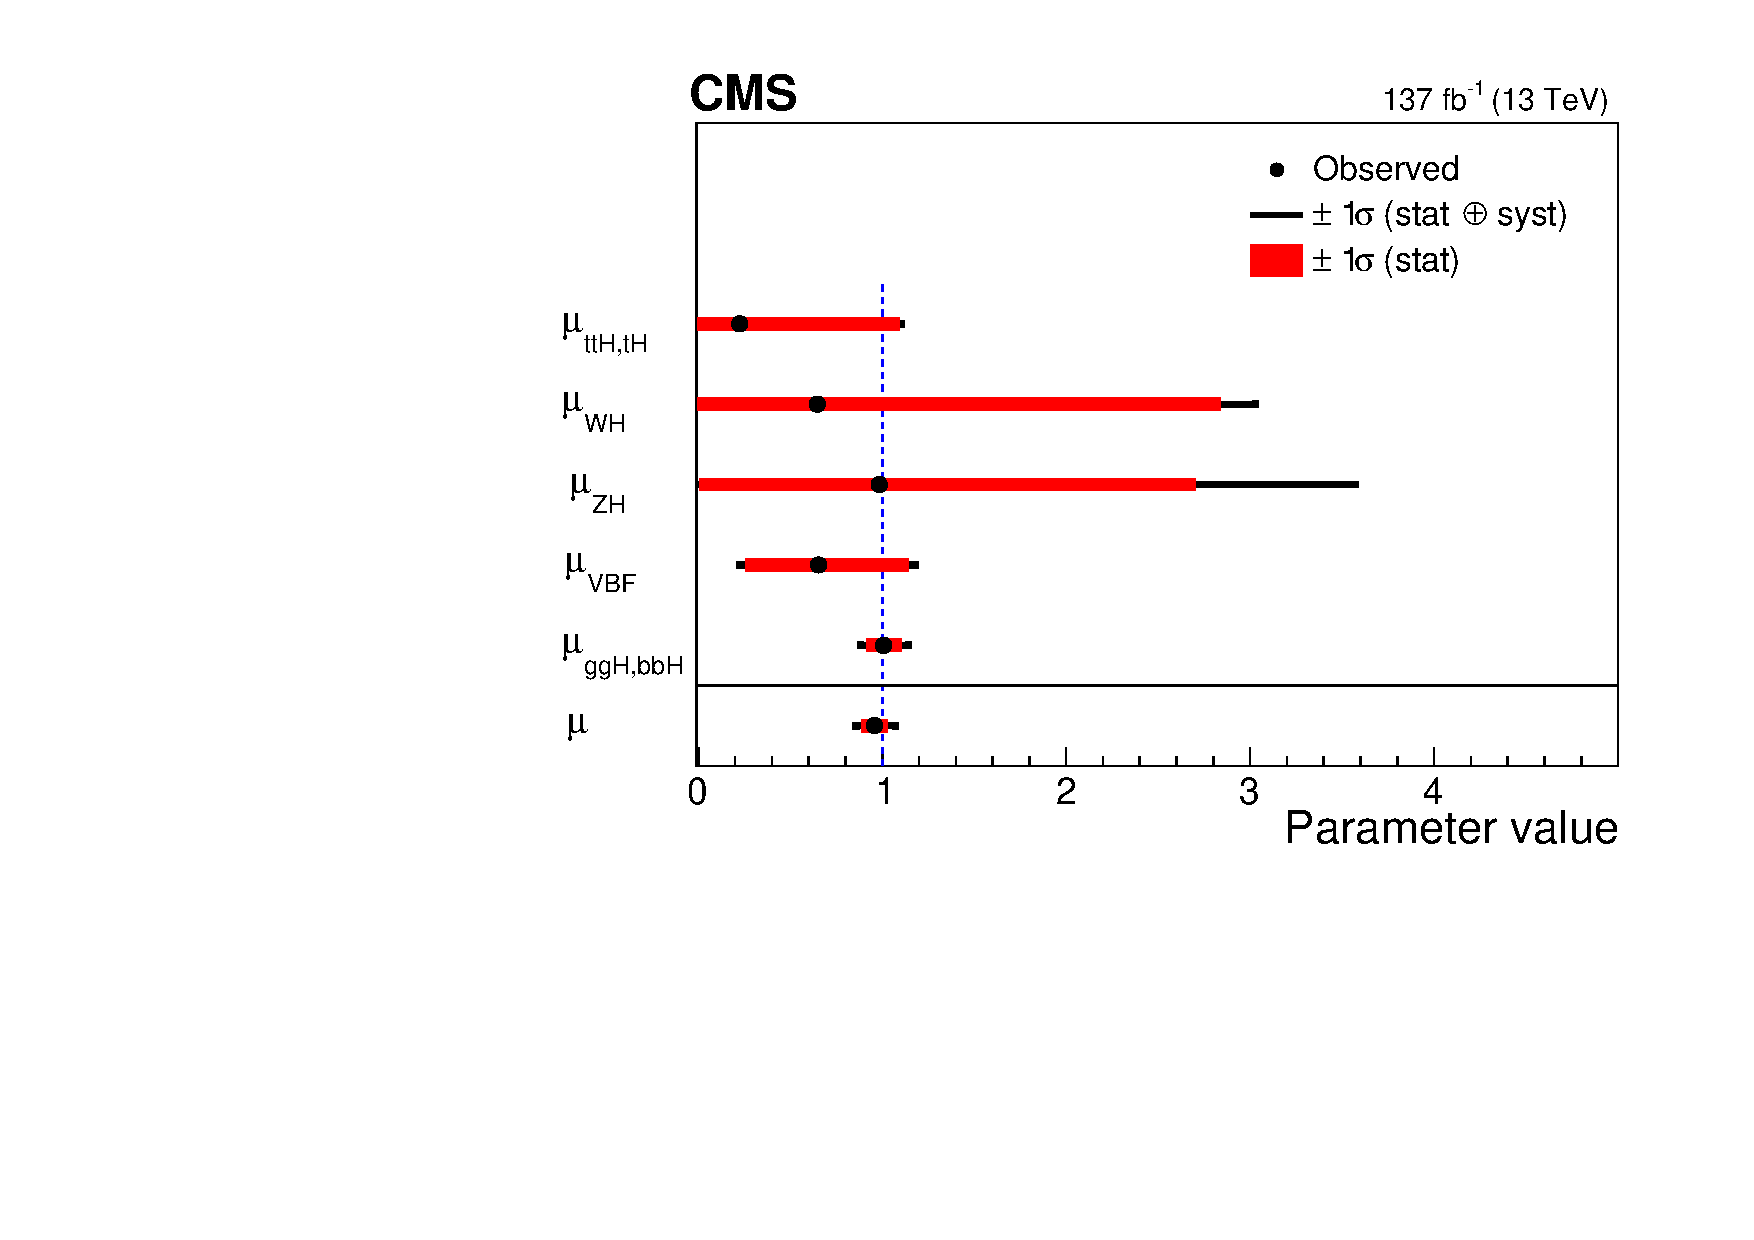
\includegraphics[width=0.45\linewidth]{Figures/results/signalstrength/mu_stage0.pdf}
%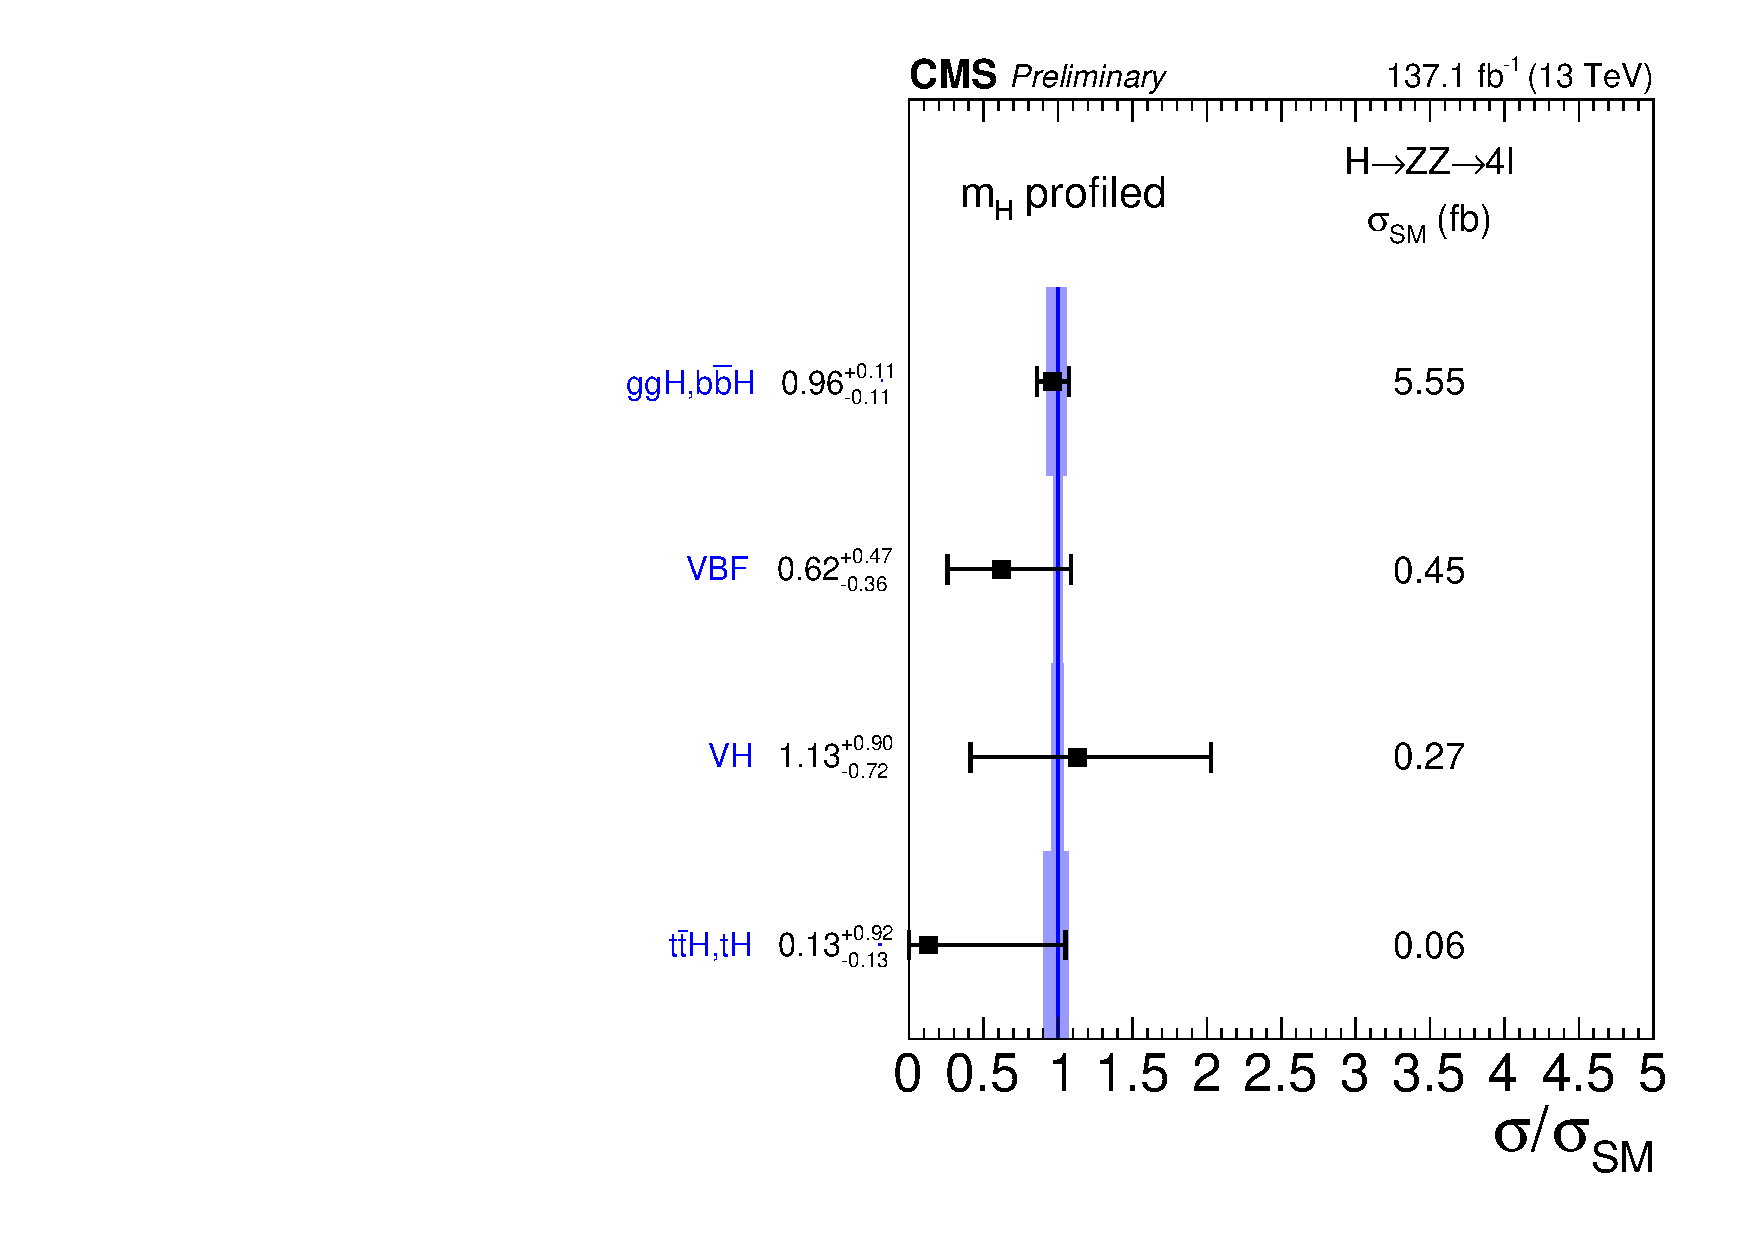
\includegraphics[width=0.45\linewidth]{Figures/results/signalstrength/mu_stage0_xsec.pdf}
%\caption{Results of likelihood scans for the signal strength modifiers (left) and cross section (right) corresponding to the four main Higgs boson production modes.
%On the left figure, the vertical line shows the combined $\mu$, together with its associated $\pm$ 1$\sigma$ uncertainties shown as filled band.  
%On the right figure, the band of the vertical line shows the theoretical uncertainties on the SM cross sections.
%The horizontal bars indicate the $\pm$ 1$\sigma$ uncertainties on $\mu$ for the different production modes. 
%The uncertainties include both statistical and systematic sources.
%\label{fig:muprocesses}}
%\end{center}
%\end{figure}
